\section{Vooronderzoek}

\subsection{wat is een neuraal netwerk}
Neurale netwerken zijn een reeks algoritmen die losjes gemodelleerd zijn van het menselijke brein. Een artificial brein dat gemaalt is uit een hele grote reeks artificial neurons.

\subsubsection{Perceptrons}
Een van de meest fundamenteele artifical neuron type word ook wel een perceptron genoemt. Een perceptron pakt verschillende binary inputs:\\ $x_{1}, x_{2},....x_{n}$ en produceerd een enkele binaire output.
\begin{center}
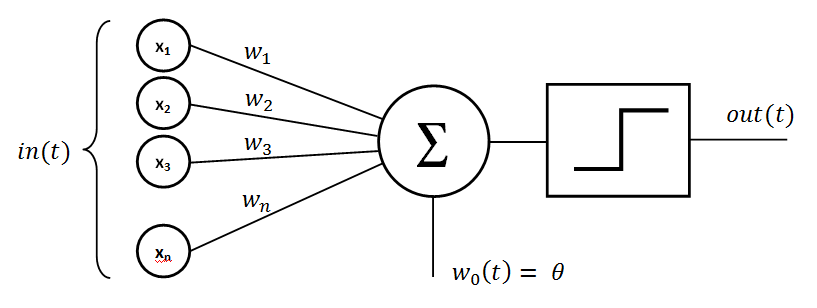
\includegraphics[scale=0.7]{perceptron.png}
\end{center}
In het voorbeeld hierboven is er een perceptron die 3 variablen als input neemt: $x_{1}, x_{2}$ en $x_{3}.$ Bij all deze waardes word een Weight toegekend($w_{n}$). Deze waarde geeft aan hoe sterk die input meeteld.\\
De perceptron neemt ook een extra input aan($w_{0}^{(t)}=\theta $) dat we de bias noemen. De bias is een waarde die de activation treshold kan verhogen of verlagen. Om de output van een perceptron the berkenen kan je deze functie gebruiken:
\begin{equation*}
\begin{rcases}
        0  if \sum_{j}w_{j}x_{j}+b \leq threshold \\
        1  if \sum_{j}w_{j}x_{j}+b > threshold
\end{rcases} 
\text{output}
\end{equation*}

\subsubsection{wat maakt een goed neuraal netwerk}

\subsubsection{wat gaat er vaak mis}

\subsection{python}

\subsection{Encog}